\documentclass[parskip=full]{scrartcl}
\usepackage[utf8]{inputenc}
\usepackage[T1]{fontenc}
\usepackage[german]{babel}
\usepackage{hyperref}
\hypersetup{ 
pdftitle={
PSE: Pflichtenheft},
bookmarks=true,
}
\usepackage{csquotes}



\begin{document}
\title{Android Go-App}
\author{Tarek, \\Dennis, \\Matthias Dressel, \\Victoria Karl, \\Theresa Heine\\
	\\Betreuer: \\Heiko Klare, \\ Erik Burger\\}
\date{\today}
\maketitle
\newpage
\tableofcontents
\newpage

\section{Einleitung}
In unserer heutigen modernen Welt ist PLANUNG das A und O, besonders bei der Organisation von Gruppentreffen. Sei es eine Wanderung im Wald, eine Kneipentour oder ein einfaches Mittagessen mit den Arbeitskollegen. Um die PLANUNG muss man sich kümmern! Nicht nur die PLANUNG ist so wichtig, sondern auch die Zeit. Man möchte so schnell wie möglich und so effektiv wie möglich PLANUNG erstellen und sich daran halten. \\
Angenommen einige Kollegen möchten ihr Mittagessen zusammen genießen, jedoch haben diese während der Arbeit kaum Zeit sich zu einigen wo  und wann man was isst. Deshalb ist es zu unserer Aufgabe geworden, diese einfache Planung zu modernisieren. Mit unserer Go-App ist es möglich eine GRUPPE zu erstellen und seine Kollegen oder Freunde in diese einzuladen. Mit einem einfach Klick werden alle in der GRUPPE informiert wo und wann man essen geht und vor allem wird den anderen in der GRUPPE angezeigt, wo man sich befindet. \\
Wir, das Team „Go-App“, haben es uns dabei zur Aufgabe gemacht, die Planung zu vereinfachen. Dabei ist unser Projekt im Rahmen eines Software-Projektes am KIT entstanden. \\

KOMMENTAR:
- "Sei es eine Wanderung im Wald, eine Kneipentour oder ein einfaches Mittagessen mit den Arbeitskollegen." ist kein echter Satz. da fehlt das Verb!!
- du brauchst nicht jeden Satz zu betonen, dass es um die Planung geht.
- Vermeide ebenfalls dopplungen wie "wo und wann"
- auch nicht "so xxx wie möglich"  2x hintereinander bringen 
- "Man möchte so schnell wie möglich und so effektiv wie möglich PLANUNG erstellen und sich daran halten." das ist doch gar nicht der Sinn der App. Vielleicht eher: Man möchte so schnell und komfortabel 	wie möglich planen können ohne sich zu sehr festlegen zu müssen.
- Angenommen    -----> Wenn zum Beispiel
- Arbeit        -----> Arbeitszeit
- versuch das "man" zu vermeiden. Das kannst du ein mal bringen, aber nicht ständig... z.B. "wo und wann sie essen wollen"     .... "wo und wann die Gruppe essen wird"
- Gruppe ist auch zu häufig hintereinander
- trenne das informiert werden und Standort anzeigen gedanklich in 2 Sätze auf... "Mit einem Klick (ein Klick ist immer einfach) werden alle Gruppenmitglieder darüber informiert, wo und wann die Gruppe essen wird. Mit einem weiteren Klick zeigen machen alle Gruppenmitglieder ihren aktuellen Standort sichtbar, womit weder treffe noch verspäten mehr ein Problem darstellt."
- der letzte Satz fällt vom Himmel. Entweder du machst da noch einen schönen Übergang, wurschtelst den oben noch mit rein, oder löscht ihn (was schade wäre, denn prinzipiell ist er nett)
- außerdem haben wir es uns wirklich zur Aufgabe gemacht "die Planung zu vereinfachen"? oder geht es nicht viel mehr darum sich leichter zu finden? D
\section{Zielbestimmung}
Die Go-App soll es Nutzern erleichtern sich in Gruppen zu organisieren
und Treffpunkte in Form von Ort und Uhrzeit festzulegen. Zu gegebenem Zeitpunkt werden die Standorte der Gruppenmitglieder und des Zielortes angezeigt.


Auf einer Karte lässt sich dabei sehen, wo sich der Zielort und die anderen Gruppenmitglieder befinden.

\subsection{Musskriterien}
\textbf{Clientseitig}
\begin{itemize}
	\item Benutzeraccount anlegen/ löschen
	\item Gruppen erstellen/ löschen
	\item Benutzer in Gruppen einladen/ aus Gruppen entfernen
	\item Gruppen beitreten/ verlassen
	\item Treffpunkte festlegen/ ändern
	\item Go-Button aktivieren/ deaktivieren
	\item Standorte von Gruppenmitgliedern anzeigen
	\item Standort des Zielortes anzeigen
\end{itemize}
\textbf{Serverseitig}
\begin{itemize}
	\item Verschlüsselung aller Personenbezogenen Daten	
\end{itemize}

\subsection{Wunschkriterien}
\begin{itemize}
	\item Änderung von Benutzer- und Gruppennamen
	\item Administratorrechte an Gruppenmitglieder übertragen
	\item Inaktive Benutzer und Gruppen löschen
	\item Go-Button und GPS-Tracking getrennt verwalten
	\item Benachrichtigungen bei Gruppenaktivität
	\item Erweiterte Verwaltung von Treffpunkten
\end{itemize}

\subsection{Abgrenzungskriterien}
\begin{itemize}
	\item GPS-Daten werden keinen Benutzern zugeordnet
	\item Es gibt keine Suchfunktion für Benutzer und Gruppen
	\item Beitreten zu Gruppen ohne den dazugehörigen Link ist nicht möglich
	\item Gruppenlinks können nicht wiederverwertet werden
	\item Abstimmungen über Ort und Uhrzeit eines Treffpunktes werden nicht unterstützt
	\item Angaben über Zu- und Absagen oder Verspätungen zu einem Treffpunkt sind nicht möglich
	\item Es lassen sich keine Nachrichten, Fotos oder andere Dateien über die App versenden
\end{itemize}
 Ta

\section{Produkteinsatz}
Das Produkt dient zur erleichterten Vermittlung zwischen Gruppenmitgliedern, um sich an einem bestimmten Zielort zu einer festgelegten Uhrzeit zu treffen. Dabei steht im Vordergrund sich gemeinsam von einer unweit entfernten Startposition auf den Weg zu machen und den Rest der Gruppe zu finden. 
Durch die anonyme Angabe der aktuellen Standorte aller Gruppenmitglieder auf der Karte, kann man so entweder auf andere warten oder diese einholen und gemeinsam den Zielort erreichen. Halten sich mehrere Mitglieder innerhalb eines Radius von 25 Metern auf, werden die Standorte dieser Mitglieder gemittelt und in Relation größer auf der Karte angezeigt, als nur der Standort eines einzelnen Mitglieds.\\

\subsection{Anwendungsbereiche}
\textbf{Privater Anwendungsbereich} \\
Im privaten Gebrauch kann das Produkt zur Verabredung zum gemeinsamen Essen oder zu anderen Freizeitaktivitäten verwendet werden. So hat jedes Mitglied Einsicht darüber, ob sich die anderen Gruppenmitglieder schon auf den Weg gemacht haben, sich verspäten werden oder wie lange sie noch brauchen um den Zielort zu erreichen.\\

\textbf{Kommerzieller Anwendungsbereich} \\
Im kommerziellen Bereich kann das Produkt seine Anwendung in der Planung von Konferenzen finden. So erfahren alle Gruppenmitglieder wo und wann die nächste Besprechung stattfindet. \\

\subsection{Zielgruppen}
Zielgruppen sind sowohl Privatpersonen als auch Unternehmen die sich in Gruppen organisieren und nicht jeden Einzelnen über einen neu anstehenden Treffpunkt informieren möchten. Bei nahe liegenden Startpositionen kommt noch hinzu, dass man sich anderen Mitgliedern anschließen und gemeinsam den Weg beschreiten kann, da deren Standorte auf der Karte sichtbar sind.\\

\subsection{Betriebsbedingungen}
Das Produkt kann bei einer bestehenden Internet- und GPS- Verbindung genutzt werden. Die GPS Technologie ist nötig um die Standorte aller Gruppenmitglieder zu erfassen und mit ausreichender Internetverbindung an die anderen Mitglieder zu übertragen. Bei Fehlen einer der beiden Komponenten ist die Funktionalität des Produkts nicht gewährleistet.\\

 Th
\section{Produktumgebung}
\subsection{Softwareanforderungen}
\subsection{Hardwareanforderungen} M
\section{Produktübersicht}
\subsection{Systemarchitektur}

\begin{figure} [h]	
	\centering
	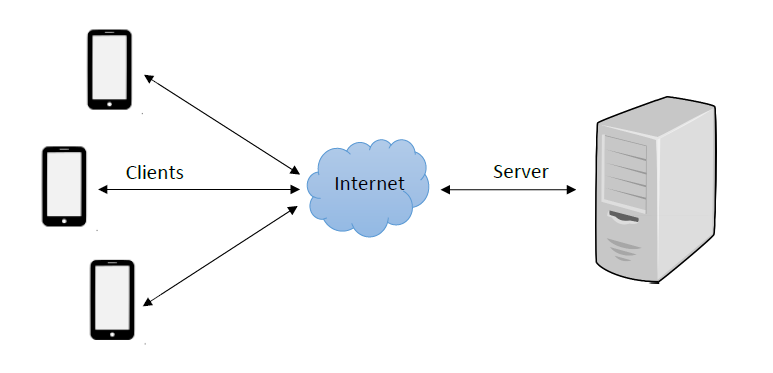
\includegraphics[scale = 0.8]{res/clientServerArchitektur.png}
\end{figure}



\subsection{Szenarien}
\subsection{Anwendungsfälle}
\subsubsection{Musskriterien}
\subsubsection{Wunschkriterien} Ta
\newpage
\section{Musskriterien}
Die Musskriterien sind in Client- und Serverseitige Interaktionen aufgeteilt.\\
\textbf{/FCXX/} steht hierbei für clientseitige Aktionen.\\
\textbf{/FSXX/} steht für die serverseitigen Reaktionen.\\
Die Nummer ist bei zusammenhängenden Aktionen gleich.\\
\subsection{Clientseitig}
     \textbf{/FC010/} Registrierung von Benutzern durch einmalige Namensfestlegung.\\
     \textbf{/FC020/} Löschen des eigenen Benutzeraccounts. Ist der Benutzer Administrator einer Gruppe oder wird eine Gruppe dadurch leer, dann wird die entsprechende Gruppe gelöscht.\\
     \textbf{/FC030/} Erstellen von Gruppen mit eindeutigem Namen. Benutzer der die Gruppe erstellt wird zum Gruppenadministrator.\\
     \textbf{/FC040/} Löschen von Gruppen (nur der Gruppenadministrator).\\
     \textbf{/FC050/} Erstellen von Gruppenlinks (nur Administrator). Diese dienen als Einladung für andere Benutzer.\\
     \textbf{/FC060/} Beitreten in eine Gruppe nur über Einladungslink (Voraussetzung registriert).\\
     Der Link wird über die Go-App geöffnet (Falls installiert).\\
     \textbf{/FC070/} Verlassen einer Gruppe (als Gruppenmitglied).\\
     \textbf{/FC080/} Entfernen von Gruppenmitgliedern (nur Gruppenadministrator): Entspricht verlassen einer Gruppe, nur erzwungen durch Gruppenadministrator.\\
     \textbf{/FC090/} Festlegen von Zielort: Einstellen von Zielort für ein Treffen (nur Gruppenadministrator).\\
     \textbf{/FC100/} Festlegen von Uhrzeit: Einstellen der Uhrzeit für ein Treffen (nur Gruppenadministrator).\\
     \textbf{/FC110/} Go-Button: Durch drücken des Go-Buttons eigene Position an die Gruppe übermitteln (alle Gruppenmitglieder).\\
     \textbf{/FC120/} Anzeigen der gemittelten GPS-Daten der Gruppe auf der Karte. Sind mehrere Mitglieder innerhalb eines bestimmten Radius,
     werden sie als Gruppe angezeigt.\\
     \textbf{/FC130/} Der Datenverkehr zwischen Client und Server wird verschlüsselt.\\
     \textbf{/FC140/} Go-Button: Durch erneutes Drücken des Go-Buttons Positionsfreigabe deaktivieren.\\
     \textbf{/FC150/} Abrufen der aktuellen Gruppenparameter vom Server bei geöffneter Go-App.\\
\subsection{Serverseitig}
     \textbf{/FS010/} Benutzername auf eindeutige ID abbilden und (Name,ID) speichern.\\
     \textbf{/FS020/} Benutzer aus allen Gruppen entfernen und das Tupel (Name, ID) vom Server löschen.\\
     \textbf{/FS030/} Eine neue Gruppe anlegen mit Gruppenadministrator als einziges Mitglied.\\
     \textbf{/FS040/} Entferne alle Mitglieder aus der Gruppe und lösche Gruppe vom Server.\\
     \textbf{/FS050/} Erstellten Gruppenlink in Gruppe speichern. Nach der Nutzung wird dieser gelöscht.\\
     \textbf{/FS060/} Link empfangen und zugehörige Gruppe identifizieren.\\ Die ID des Benutzers wird dann der Gruppenliste hinzugefügt und der genutzte Link gelöscht.\\
     \textbf{/FS070/} Löschen der ID des Benutzers der die Gruppe verlässt aus der Gruppenliste.\\
     \textbf{/FS090/} Parameter für den Zielort empfangen und in der Gruppe speichern.\\
     \textbf{/FS100/} Für den Parameter 'Uhrzeit' wird genauso verfahren wie in /FS090/. \\
     \textbf{/FS110/} Position als GPS Koordinaten empfangen und zwischenspeichern.\\
     \textbf{/FS120/} Bei Anfrage aktuelle GPS-Daten der Mitglieder an Mitglied senden.\\
     \textbf{/FS130/} Der Datenverkehr von Server zu Client wird verschlüsselt.\\
     \textbf{/FS150/} Bei Anfrage: Senden der aktuellen Gruppenparameter inklusive Status der Gruppenmitglieder.\\
\section{Wunschkriterien}
\subsection{Clientseitig}
     \textbf{/FC160/} Benutzung des Go-Buttons bei deaktiviertem GPS.\\
     \textbf{/FC170/} Änderung des Benutzernamens nach erstmaliger Registrierung.\\
     \textbf{/FC180/} Gruppenmitglieder zu Administratoren machen.\\
     \textbf{/FC190/} Änderung des Gruppennamens nach Erstellen der Gruppe.\\
     \textbf{/FC200/} Benutzer nach langer Inaktivität löschen. Wird eine Gruppe dadurch leer: Gruppe löschen.\\
     \textbf{/FC210/} Anzeigen der Namen von Gruppenmitgliedern, die den Go-Button schon gedrückt haben.\\
     \textbf{/FC220/} Benachrichtigung über das 'Aufbrechen' anderer Gruppenmitglieder.\\
     \textbf{/FC230/} Benachrichtigung bei Änderung eines Treffpunkt Parameters (Ort/Uhrzeit).\\
     \textbf{/FC240/} Treffpunkte für ein spezielles Datum festlegen.\\
\subsection{Serverseitig}
     \textbf{/FS170/} Einer Benutzer-ID einen neuen Namen zuordnen.\\
     \textbf{/FS180/} Bei einem Benutzer in einer Gruppenliste das Admin-Flag setzen.\\
     \textbf{/FS190/} Überprüfen ob Gruppenname vergeben ist und ändern.\\
     \textbf{/FS200/} Regelmäßig überprüfen wann ein Nutzer zuletzt aktiv war.\\
     \textbf{/FS210/} Go-Button Event von Gruppenmitglied empfangen und alle anderen Gruppenmitglieder benachrichtigen.\\
     \textbf{/FS220/} Gleiches Prinzip wie beim vorherigen Punkt bei Veränderung der Gruppenparameter.\\
 Ta, Th
\section{Produktdaten}

Die Speicherung aller hier genannten Daten erfolgt, soweit nicht anders spezifiziert, auf dem Server des Dienstes.

\textbf{Über die Benutzer ist zu speichern:}\\

\textbf{/PD010/}Dem Endgerät des Benutzers wird eine Identifikationsnummer zugeordnet und in Verknüpfung mit dem Benutzername gespeichert. Zusätzlich wird der
 Benutzername auch noch auf dem Endgerät gespeichert.

\textbf{/PD020/}Der Standort des Endgerätes wird in Verknüpfung mit der Identifikationsnummer von diesem gespeichert.

\textbf{/PD030/}Der Gruppenname wird gespeichert und zur Identifikation verwendet.

\textbf{/PD040/}Sowohl auf dem Server als auch auf dem Endgerät des Gruppenadministrators wird eine Verknüpfung erstellt und gespeichert, um dieses Gruppenmitglied als Gruppenadministrator zu kennzeichnen.

\textbf{/PD050/}Die versendeten Links werden mit dem Gruppennamen verknüpft und gespeichert. 

\textbf{/PD060/}Die Identifikationsnummer des Benutzers wird mit dem Gruppennamen verknüpft und gespeichert.

\textbf{/PD070/}Zielort und Uhrzeit werden zusammen mit dem Gruppennamen verknüpft und gespeichert. V
\section{Produktleistungen/ Qualitätsziele}
\textbf{Stabilität:}\\
/LXXX/	Es müssen insgesamt maximal 100.000 User und maximal 50.000 Gruppen verwaltet werden. \\
/LXXX/	Es sind maximal 200 User und maximal 100 Gruppen gleichzeitig aktiv \\
/LXXX/	Sollte kein Datenabgleich mit dem Server möglich sein, so sind die Daten dennoch  auf den jeweiligen Geräten abgespeichert.	  \\
\textbf{Datensicherheit:}\\
/LXXX/	Daten werden während der Datenübertragung ausreichend verschlüsselt\\
/LXXX/	Verschlüsselungsdaten müssen klein gehalten werden, um System Skalierbarkeit zu ermöglichen\\
/LXXX/	Passwörter müssen mindestens 6 stetig sein.\\
\textbf{Benutzbarkeit:}\\
/LXXX/	Server Reaktionszeit bei (Gruppen erstellung) darf nicht länger als 15 Sekunden dauern\\
/LXXX/	Server Reaktionszeit bei (Profil Erstellung - also registierung) darf nicht länger als 15 Sekunden dauern\\
/LXXX/	Die GPS Standort Übermittlung muss eine Genauigkeit von maximal 10 Metern haben\\
/LXXX/	Die GPS Standort Übermittlung darf nicht länger als 5 Sekunden sein  \\
/LXXX/	Datenübertragung zum Server dauern im Schnitt nicht länger als 10 Sekunden\\
/LXXX/	Namen sind nicht eindeutig und sind änderbar\\
/LXXX/	Gruppen Namen sind nicht eindeutig und sind änderbar\\ D
%KOMMENTAR ZUM GESAMTEN DOKUMENT
%- Du musst in deinen Beschreibungen auch nicht davon ausgehen, dass du die App jemandem erklärst, der noch nie eine App verwendet hat. So knapp  und übersichtlich wie möglich ist dein Ziel. Viel Text bedeutet, unsere App ist zu kompliziert, dass wir jede Menge Text zum erklären brauchen. 
%-achte drauf, dass du bei Beschreibung, Elemente und Verwendung nichts doppelt schreibst... das ist ein paar mal zu 80% dasselbe
%-das Wort "Tippen" so gut wie möglich vermeiden

%- ich muss sagen, dass es sehr anstrengend ist den Text zu lesen, dabei sollte es kurz und knackig und informativ sein. Ich fühl mich eher, wie wenn ich grade 100 mal dasselbe gelesen habe und hatte gegen Ende keine Lust mehr bzw. war mir schon sicher zu wissen, was drin steht. 

\section{Benutzerschnittstelle}
\begin{wrapfigure}{l}{0.35\textwidth}
	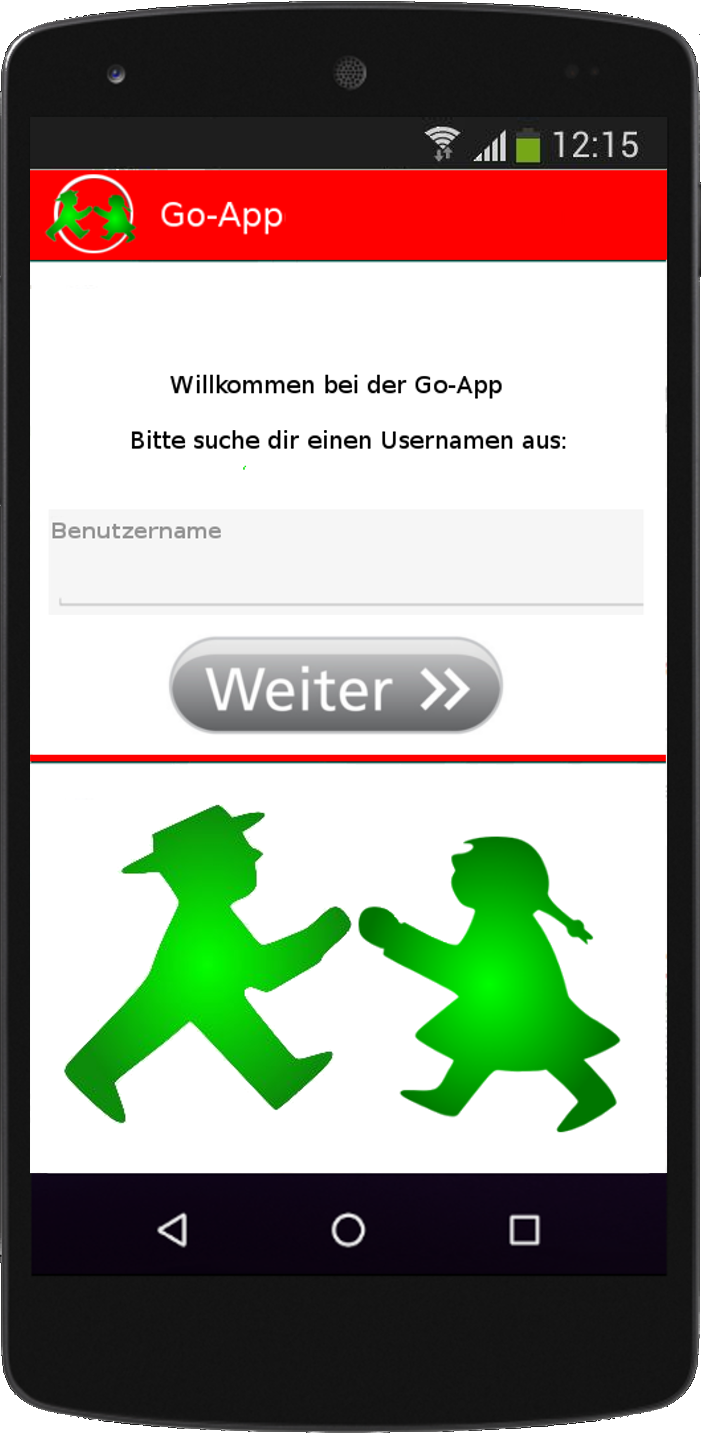
\includegraphics[scale=0.2]{resources/images/handy/startansicht.png}
	\caption{Erste Startansicht}
\end{wrapfigure}


\textbf{Beschreibung:}\\
Erste Startansicht der Go-App, Aufforderung an den neuen Benutzer einen Benutzernamen zu wählen.\\
\textbf{Elemente:}\\
Textfeld "Benutzername" zum Einfügen des Benutzernamens.\\
"Weiter"-Button um diesen zu bestätigen.\\
\textbf{Verwendung:}\\
Durch einmaliges Tippen auf das Textfeld "Benutzername" wird die Bildschirmtastatur aktiviert und der Benutzer kann seinen gewählten Benutzernamen eingeben.\\
Durch einmaliges Tippen auf den "Weiter"-Button wird dieser Benutzername bestätigt und der Benutzer wird zur Gruppenübersicht weitergeleitet.

%\\
%-KOMMENTAR
%--"tippen" brauchst du nicht verwenden. Schreib einfach: Im Textfeld "Username" wird die Bildschirmtastatur aktiviert...
\clearpage
\newpage

\begin{wrapfigure}{l}{0.35\textwidth}
	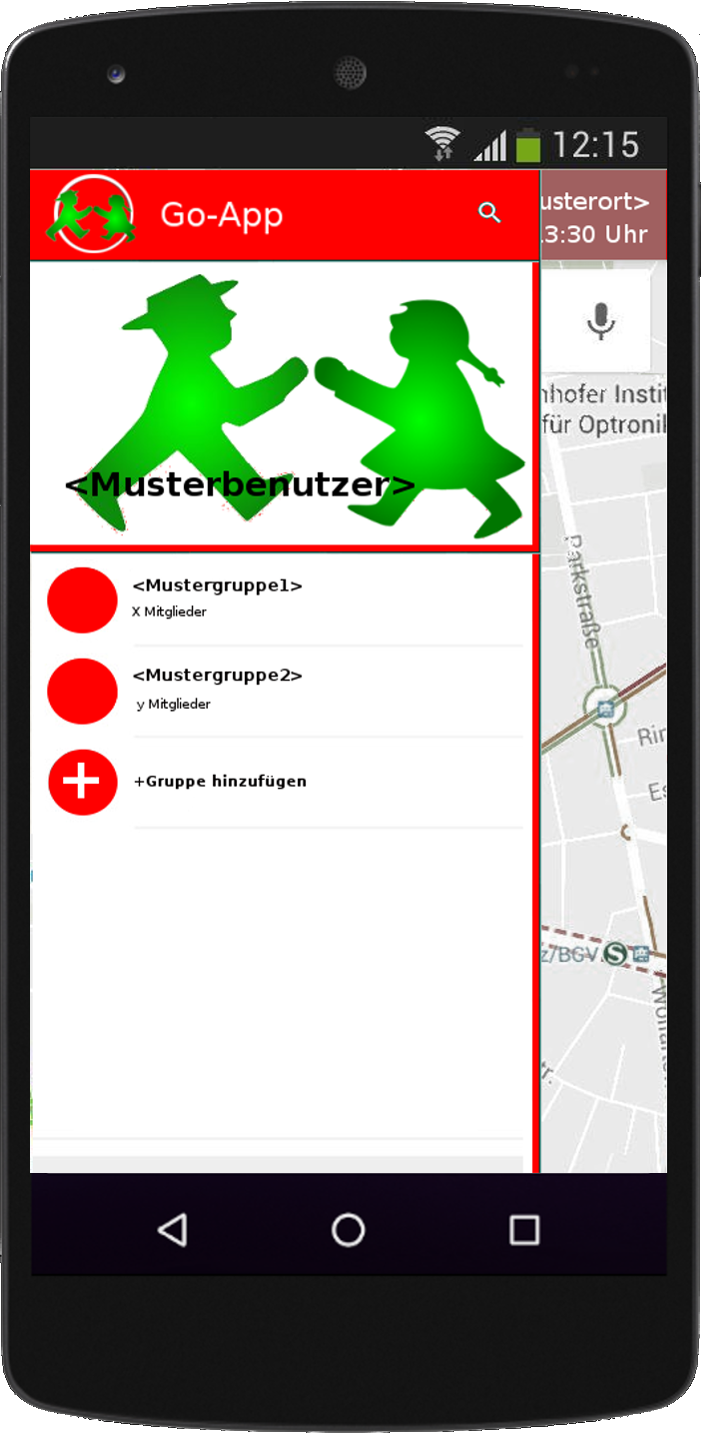
\includegraphics[scale=0.2]{resources/images/handy/gruppenuebersicht.png}
	\caption{Gruppenübersicht}
\end{wrapfigure}

%\begin{minipage}[t]{0.8\textwidth}
%\begin{figure}[t]
	%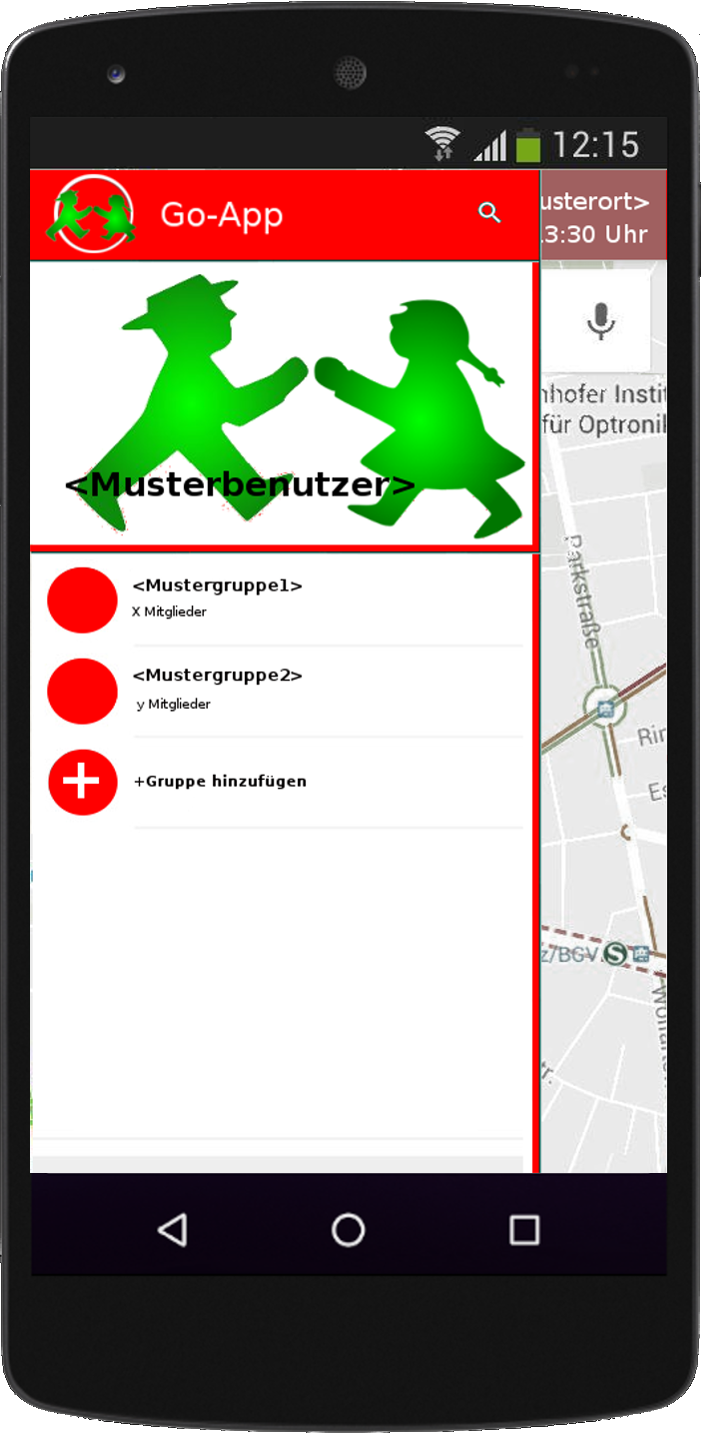
\includegraphics[width=0.2\textwidth]{resources/images/handy/gruppenuebersicht.png}
	%\caption{Gruppenübersicht}
%\end{figure}
%\end{minipage}

%\begin{wrapfigure}{l}{0.35\textwidth}
	%\begin{center}
	%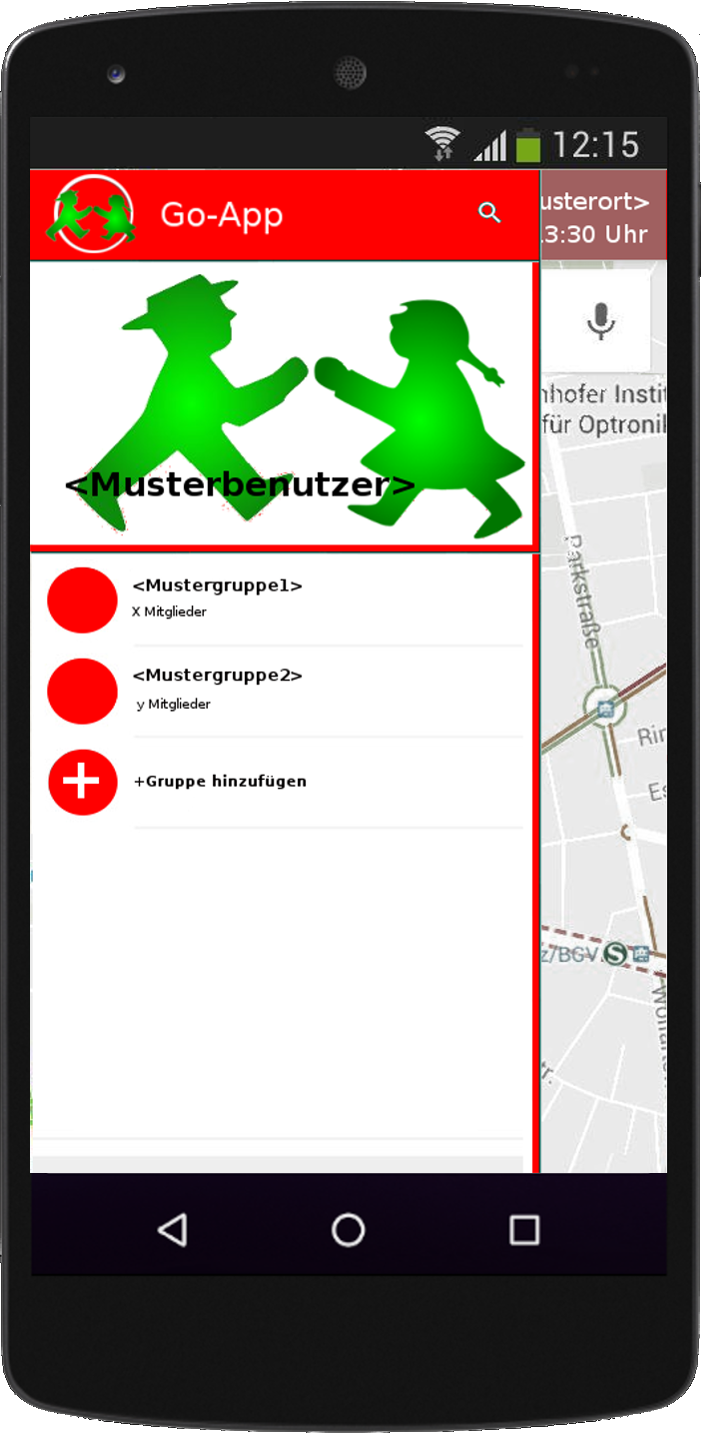
\includegraphics[scale=0.2]{resources/images/handy/gruppenuebersicht.png}
	%\caption{Gruppenübersicht}
	%\end{center}
%\end{wrapfigure}

\textbf{Beschreibung:}\\
Übersicht über die Gruppen, in denen der Benutzer Mitglied ist. Wenn dieser das erste Mal zu der angegebenen Ansicht gelangt, ist er noch kein Mitglied einer Gruppe und deshalb werden ihm auch noch keine angezeigt.\\
\textbf{Elemente:}\\
Benutzernahme zur Orientierung, mit welchem Namen der Benutzer registriert ist.\\
Gruppennamen zur Übersicht über die Gruppen, in denen der Benutzer Mitglied ist.\\
"Gruppe hinzufügen"-Button um eine neue Gruppe hinzuzufügen.\\
\textbf{Verwendung:}\\
WK(Wunschkriterium): Durch einmaliges Tippen auf den Benutzernamen wird der Benutzer weitergeleitet zur Option Benutzername ändern.\\
Durch einmaliges Tippen auf einen Gruppennamen wird der Benutzer weitergeleitet zur Kartenansicht der Gruppe.\\
Durch langes Tippen auf einen Gruppennamen kann der Benutzer "aus der Gruppe austreten" wählen bzw. der GA (Gruppenadministrator) "Gruppe löschen".\\
Durch einmaliges Tippen auf den "Gruppe hinzufügen"-Button wird der Benutzer weitergeleitet zur Option "Gruppe hinzufügen".\\
Durch Streichen nach oben oder unten kann der Benutzer durch die Gruppen scrollen, wenn es mehr sind als auf den Bildschirm passen.\\
Durch Streichen von rechts nach links kann man die Gruppenansicht weg schieben und gelangt zu der zuletzt verwendeten Karte.
\clearpage
\newpage

%KOMMENTAR
%-ich würde die Wörter Button soweit als möglich vermeiden und einfach: über "Gruppe hinzufügen" kann eine neue Gruppe erstellt werden
%-auch hier würde ich Tippen so gut wie möglich wieder weglassen, nur wenn es wirklich wichtig ist. Und ich glaube langes Tippen gibt es nicht... zumindest hört es sich komisch 

\begin{wrapfigure}{l}{0.35\textwidth}
	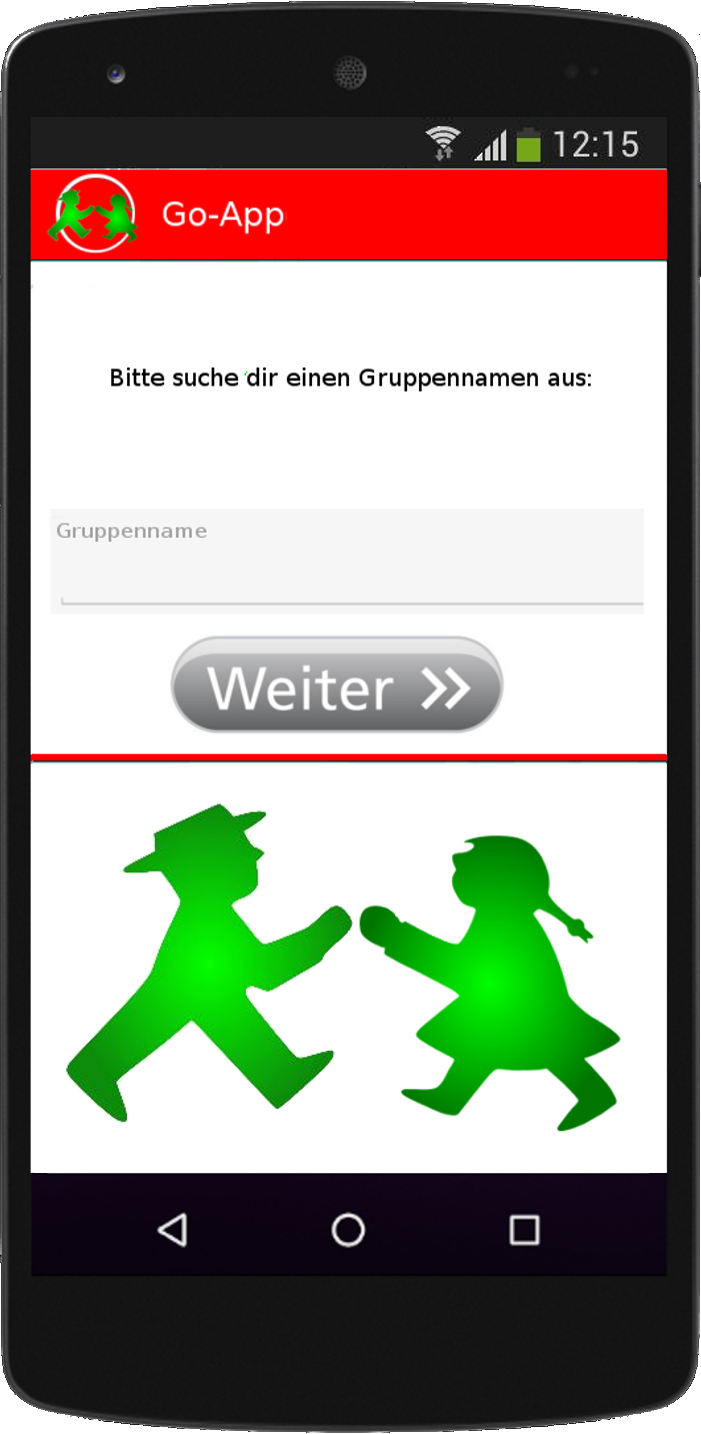
\includegraphics[scale=0.2]{resources/images/handy/gruppe_erstellen.png}
	\caption{Gruppe erstellen}
\end{wrapfigure}

\textbf{Beschreibung:}\\
Option Gruppe hinzufügen, Aufforderung an den Benutzer sich einen Gruppennamen zu wählen.\\
\textbf{Elemente:}\\
Textfeld "Gruppenname" zum Einfügen des Gruppennamens.\\
"Weiter"-Button um diesen zu bestätigen.\\
\textbf{Verwendung:}\\
Durch einmaliges Tippen auf das Textfeld "Gruppenname" wird die Bildschirmtastatur aktiviert und der Benutzer kann seinen gewählten Gruppennamen eingeben.\\
Durch einmaliges Tippen auf den "Weiter"-Button wird dieser Gruppenname überprüft. Ist dieser noch nicht vergeben, wird er bestätigt und der Benutzer wird weitergeleitet zur Gruppenübersicht. Gibt es bereits eine Gruppe die den gewählten Namen trägt, wird der Benutzer aufgefordert einen anderen Gruppennamen auszuwählen.
\clearpage
\newpage

\begin{wrapfigure}{l}{0.35\textwidth}
	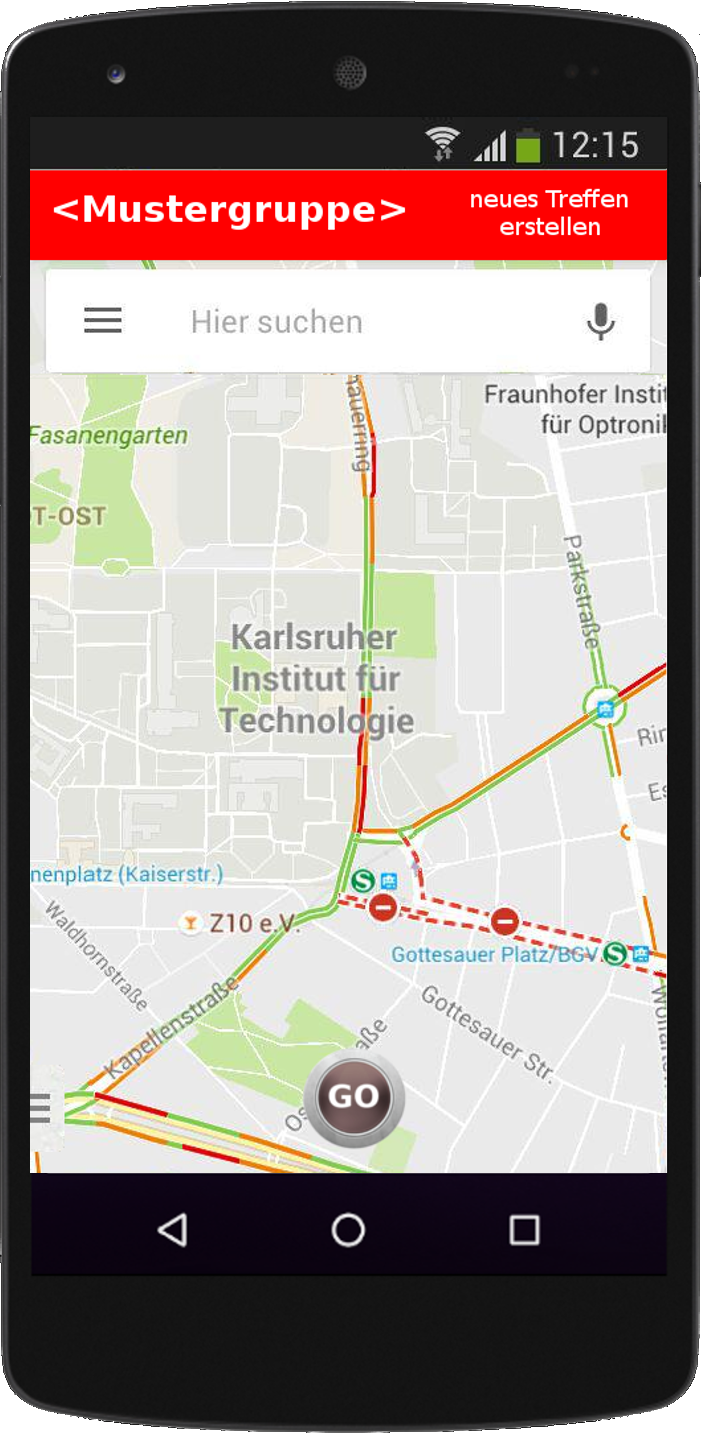
\includegraphics[scale=0.2]{resources/images/handy/map_leer_admin.png}
	\caption{Karten-Ansicht der Gruppe (leer)}
\end{wrapfigure}

\textbf{Beschreibung:}\\
Kartenansicht der Gruppe. Wenn der GA(Gruppenadministrator) das erste Mal zu dieser Ansicht gelangt, hat er noch keine Treffen erstellt und somit wird ihm auch noch eine leere Karte angezeigt. Ebenso wenn er kein aktuelles Treffen erstellt hat, wird allen GM(Gruppenmitgliedern) eine leere Karte angezeigt.\\
\textbf{Elemente:}\\
"Gruppenname"-Button um zu den Gruppendetails zu gelangen.\\
"neues Treffen erstellen"-Button bei der Ansicht des GA um ein neues Treffen zu erstellen, bzw. "kein aktuelles Treffen"-Anzeige bei der Ansicht aller GM ohne besondere Rechte.\\
"Hier suchen"-Textfeld um einen Ort auf der Karte zu suchen.\\
Handle links unten in der Ecke um die Gruppenansicht wieder herauszuziehen.\\
"Go"-Button ausgegraut bei Inaktivität.\\
\textbf{Verwendung:}\\
Durch einmaliges Tippen auf den "Gruppenname"-Button wird das GM weiter geleitet zu der Ansicht "Gruppendetails".\\
Durch einmaliges Tippen auf den "neues Treffen erstellen"-Button wird der GA weiter geleitet zu der Option "Treffen erstellen", für alle anderen GM ist diese "kein aktuelles Treffen"-Anzeige lediglich informativ.\\
Durch einmaliges Tippen auf das Textfeld "Hier suchen" wird die Bildschirmtastatur aktiviert und das GM kann seinen gewählten Ort eingeben.\\
Durch Streichen von links nach rechts über den Handle-Button kann das GM die Gruppenansicht wieder herausziehen.
\clearpage
\newpage

%KOMMENTAR
%-du erklärst teilweise bei Elemente schon, was diese machen und dann bei Verwendung nochmal: "neues Treffen erstellen"-Button bei der Ansicht des GA um ein neues Treffen zu erstellen"
%Durch einmaliges Tippen auf den "neues Treffen erstellen"-Button wird der GA weiter geleitet zu der Option "Treffen erstellen"
\begin{wrapfigure}{l}{0.35\textwidth}
	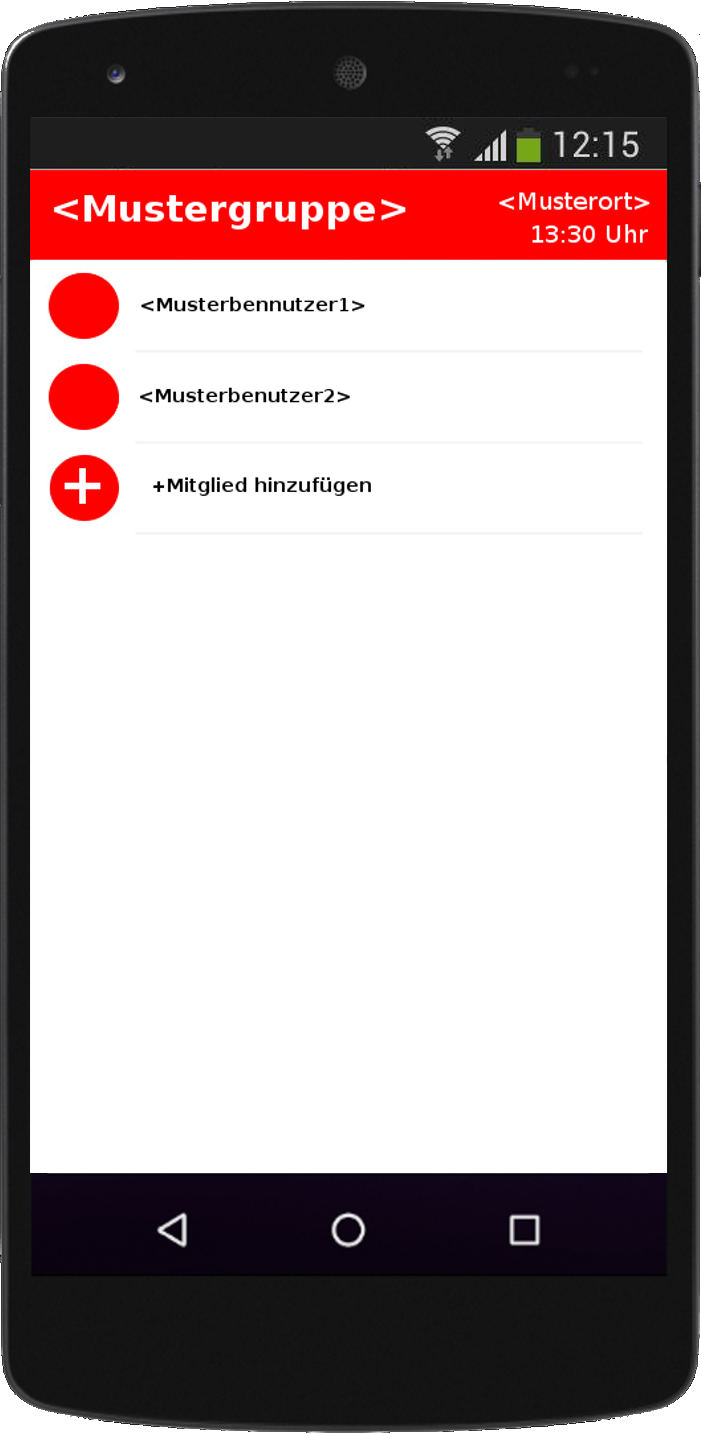
\includegraphics[scale=0.2]{resources/images/handy/gruppendetails_admin.png}
	\caption{Übersicht über die Gruppenmitglieder}
\end{wrapfigure}

\textbf{Beschreibung:}\\
Übersicht über die GMer. Wenn der GA das erste Mal zu dieser Ansicht gelangt, ist außer ihm noch kein weiteres Mitglied in dieser Gruppe.\\
\textbf{Elemente:}\\
"Gruppenname"-Button zur Übersicht, in welcher Gruppe das GM aktiv ist und um zurück zur Karten-Ansicht der Gruppe zu gelangen.\\
"neues Treffen erstellen"-Button oder "Uhrzeit"-Button bei der Ansicht des GA um ein neues Treffen zu erstellen, bzw. "kein aktuelles Treffen"-Anzeige oder "Uhrzeit"-Anzeige bei der Ansicht aller GMG ohne besondere Rechte.\\
Mitgliedernamen zur Übersicht über die Mitglieder der Gruppe.\\
"Mitglied hinzufügen"-Button um ein neues GM einzuladen aus Ansicht des GA.\\
\textbf{Verwendung:}\\
Durch einmaliges Tippen auf den "Gruppenname"-Button wird der Gruppenadministrator zurück geleitet zu der Kartenansicht der Gruppe.\\
"neues Treffen erstellen"-Button bzw. Uhrzeit-Button hat die selbe Funktion wie in der Kartenansicht der Gruppe.\\
Durch einmaliges Tippen auf den "Mitglied hinzufügen"-Button öffnet sich das Fenster "Link versenden".
\clearpage
\newpage

%KOMMENTAR
%-in welcher Gruppe man gerade aktiv ist, sieht man doch schon am Gruppennamen, da muss man doch nicht erst noch drauf gehen und nachschauen (oder was sieht man da was man nicht schon am Gruppennamen sieht)

\begin{wrapfigure}{l}{0.35\textwidth}
	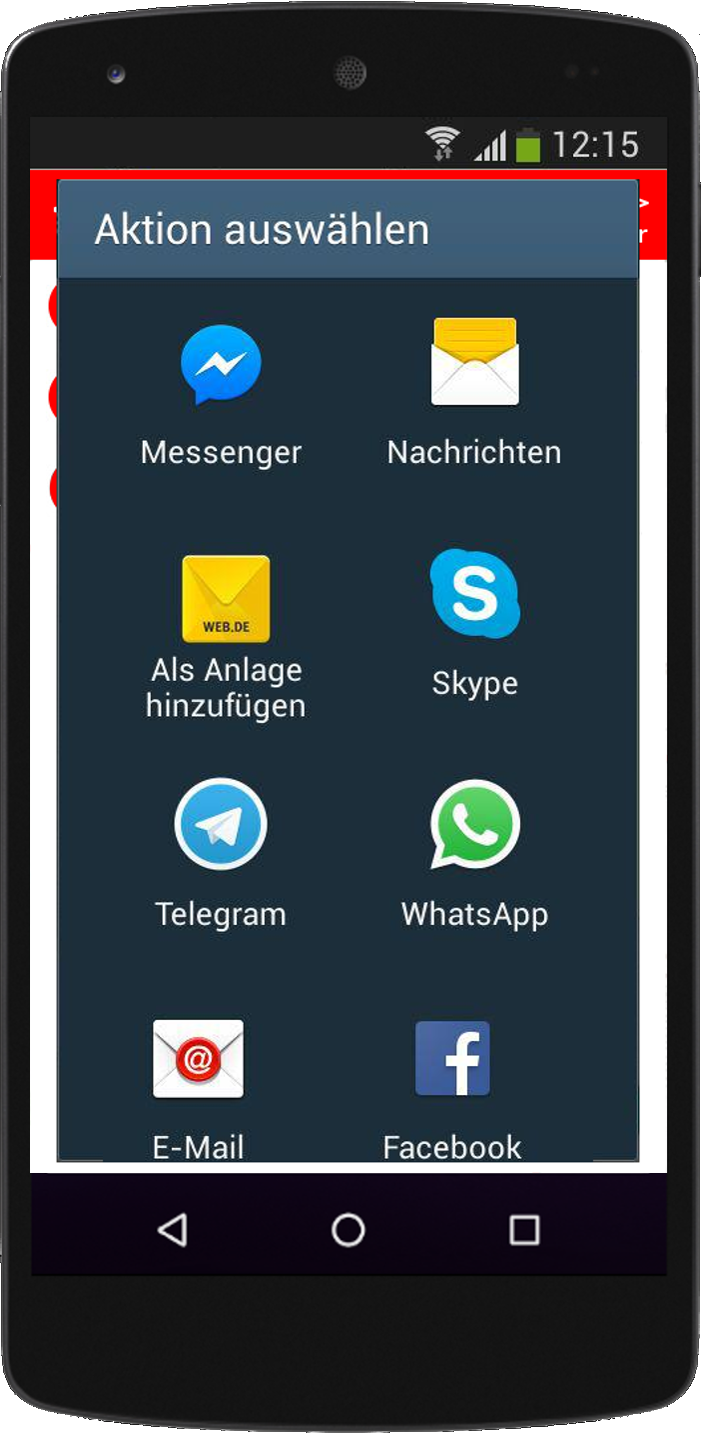
\includegraphics[scale=0.2]{resources/images/handy/link_versenden.png}
	\caption{Link versenden}
\end{wrapfigure}

\textbf{Beschreibung:}\\
Übersicht über verschiedene Kommunikationswege, die verwendet werden können um andere GM in die Gruppe einzuladen.\\
\textbf{Elemente:}\\
Auswahlmöglichkeiten der Kommunikationswegen, die der GA auf seinem Android-Gerät installiert hat.\\
\textbf{Verwendung:}\\
Durch einmaliges Tippen auf einen der Buttons wird der GA weitergeleitet zu der ausgewählten Applikation über die er dann den neu generierten Gruppen-Einladungs-Link versenden kann.
\clearpage
\newpage

\begin{wrapfigure}{l}{0.35\textwidth}
	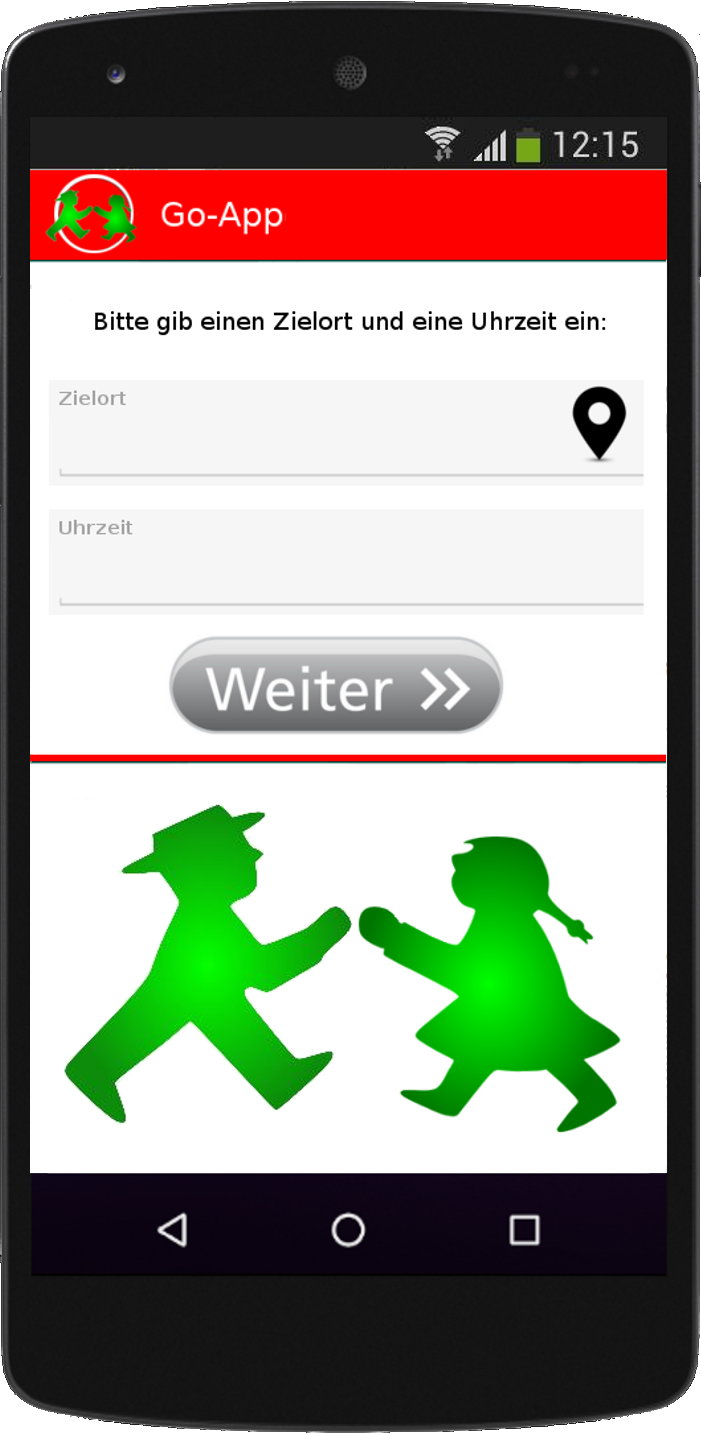
\includegraphics[scale=0.2]{resources/images/handy/treffpunkt_erstellen.png}
	\caption{Treffen erstellen}
\end{wrapfigure}

\textbf{Beschreibung:}\\
Option zum Erstellen eines neuen Treffens, Aufforderung an den Gruppenadministrator einen Zielort und eine Uhrzeit zu wählen.\\
\textbf{Elemente:}\\
Textfeld "Zielort" zum Einfügen des Zielortes.\\
Karten-Symbol-Button zum Auswählen des Zielortes per Karte.\\
Textfeld "Uhrzeit" zum Einfügen der Uhrzeit.\\
"Weiter"-Button um diese zu bestätigen.\\
\textbf{Verwendung:}\\
Durch einmaliges Tippen auf das Textfeld "Zielort" wird die Bildschirmtastatur aktiviert und der GA kann seinen gewählten Zielort eingeben.\\
Alternativ: durch einmaliges Tippen auf den Karten-Symbol-Button wird der GA weitergeleitet zu der Kartenansicht und kann dort durch einmaliges Tippen auf einen Ort diesen als Zielort eingeben.\\
Durch einmaliges Tippen auf das Textfeld "Uhrzeit" wird die Bildschirmtastatur aktiviert und der GA kann seine gewählte Zielzeit eingeben.\\
Durch einmaliges Tippen auf den "Weiter"-Button werden dieser Zielort und diese Uhrzeit überprüft. Sind die Eingaben zulässig, werden diese bestätigt und der Gruppenadministrator wird weitergeleitet zu der Kartenansicht der Gruppe. Sind Zielort und Uhrzeit nicht gültig, wird der GA aufgefordert einen anderen Ort, bzw. eine andere Zeit auszuwählen
\clearpage
\newpage

%KOMMENTAR
%- siehe Anfangskommentare oder die von den anderen 


\begin{wrapfigure}{l}{0.35\textwidth}
	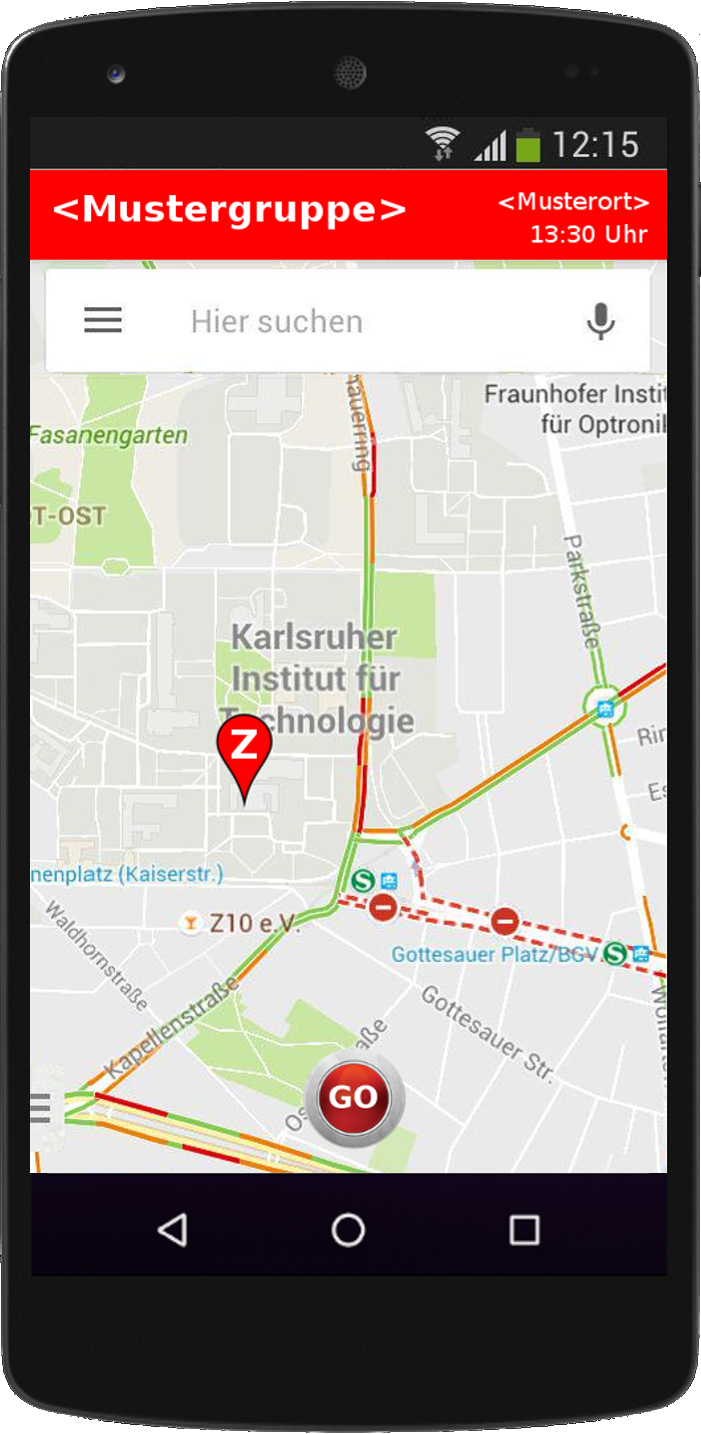
\includegraphics[scale=0.2]{resources/images/handy/map.png}
	\caption{Karten-Ansicht der Gruppe}
\end{wrapfigure}

\textbf{Beschreibung:}\\
Kartenansicht der Gruppe mit festgelegtem Treffpunkt. Allen GMern wird in dieser Ansicht nicht nur die Karte angezeigt, sondern auch der Zielort und die Uhrzeit des nächsten festgelegten Treffpunktes, außerdem noch auf der Karte der Zielort durch eine Stecknadel beschriftet mit "Z".\\
\textbf{Elemente:}\\
"Gruppenname"-Button um zu den Gruppendetails zu gelangen.\\
"Zielort - Uhrzeit"-Ansicht zur Orientierung wann und wo das nächste Treffen statt findet, bzw. "Zielort - Uhrzeit"-Button bei der Ansicht des GA um ein neues Treffen zu erstellen.\\
"Hier suchen"-Textfeld um einen Ort auf der Karte zu suchen.\\
Handle links unten in der Ecke um die Gruppenansicht wieder herauszuziehen.\\
Aktivierter "Go"-Button um anzuzeigen, wann man los geht.
\textbf{Verwendung:}\\
Durch einmaliges Tippen auf den "Gruppenname"-Button wird das GM weiter geleitet zu der Ansicht "Gruppendeteils".\\
Durch einmaliges Tippen auf den "Zielort - Uhrzeit"-Button wird der GA weiter geleitet zu der Option "Treffen erstellen".\\
Durch einmaliges Tippen auf das Textfeld "Hier suchen" wird die Bildschirmtastatur aktiviert und das GM kann seinen gewählten Ort eingeben.\\
Durch Streichen von links nach rechts über den Handle-Button kann das GM die Gruppenansicht wieder herausziehen.\\
Durch einmaliges Tippen auf den "Go"-Button sendet das GM seinen Standort in regelmäßigen Zeitabständen zu den anderen GM und erhält auch alle nötigen Informationen über diese (Ansicht: "Kartenansicht der Gruppe - treffen").
\clearpage
\newpage

\begin{wrapfigure}{l}{0.35\textwidth}
	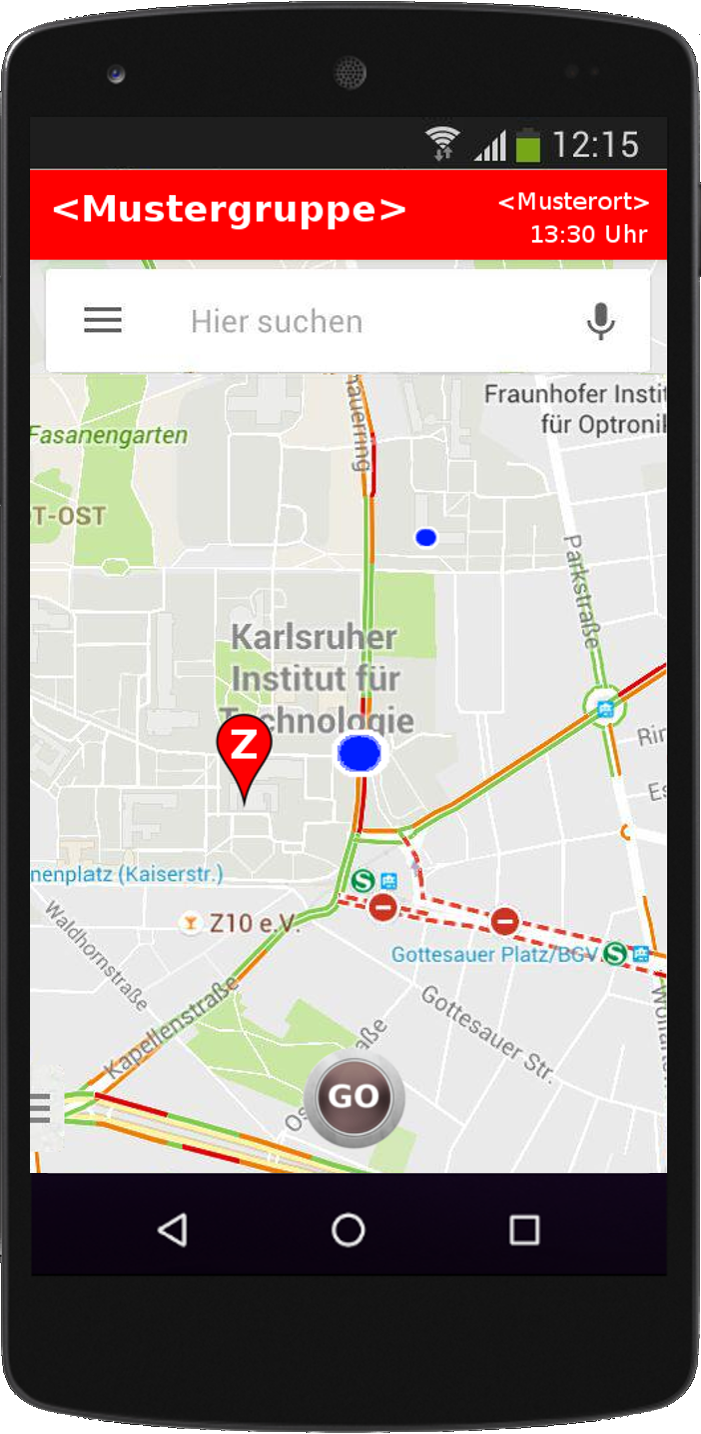
\includegraphics[scale=0.2]{resources/images/handy/map_go.png}
	\caption{Karten-Ansicht der Gruppe - treffen}
\end{wrapfigure}

\textbf{Beschreibung:}\\
Kartenansicht der Gruppe wenn der "Go"-Button schon gedrückt ist. Allen GM wird in dieser Ansicht nicht nur die Karte angezeigt, sondern auch der Zielort und die Uhrzeit des nächsten festgelegten Treffpunktes, außerdem noch auf der Karte der Zielort durch eine Stecknadel beschriftet mit "Z" und die Standorte der anderen GMer durch blaue Kreise. Je größer ein Kreis, desto mehr GM befinden sich an dem gleichen Standort.\\
\textbf{Elemente:}\\
"Gruppenname"-Button um zu den Gruppendetails zu gelangen.\\
"Zielort - Uhrzeit"-Ansicht zur Orientierung wann und wo das nächste Treffen festgelegt ist, bzw. "Zielort - Uhrzeit"-Button bei der Ansicht des GA um ein neues Treffen zu erstellen.\\
"Hier suchen"-Textfeld um einen Ort auf der Karte zu suchen.\\
Lupen-Button um die Suche zu starten.\\
Handle links unten in der Ecke um die Gruppenansicht wieder herauszuziehen.\\
Deaktivierter "Go"-Button um das Versenden des eigenen Standortes zu stoppen.\\
Blaue Kreise zur Orientierung, wo sich die anderen GM befinden.\\
\textbf{Verwendung:}\\
Durch einmaliges Tippen auf den "Gruppenname"-Button wird das GM weiter geleitet zu der Ansicht "Gruppendeteils".\\
Durch einmaliges Tippen auf den "Zielort - Uhrzeit"-Button wird der GA weiter geleitet zu der Option "Treffen erstellen".\\
Durch einmaliges Tippen auf das Textfeld "Hier suchen" wird die Bildschirmtastatur aktiviert und das GM kann seinen gewählten Zielort eingeben.\\
Durch einmaliges Tippen auf den Lupen-Button wird eine Suche nach dem gewählten Zielort gestartet und die Ergebnisse dem GM angezeigt.\\
Durch Streichen von links nach rechts über den Hanlde-Button kann das GMG die Gruppenansicht wieder herausziehen.\\
Durch einmaliges Tippen auf den "Go"-Button wird dieser deaktiviert und das Senden des Standortes des GM wird gestoppt. Außerdem kann das GM dann nicht mehr die Standorte der anderen GM sehen (Ansicht: "Kartenansicht der Gruppe").
\clearpage
\newpage


\begin{wrapfigure}{l}{0.35\textwidth}
	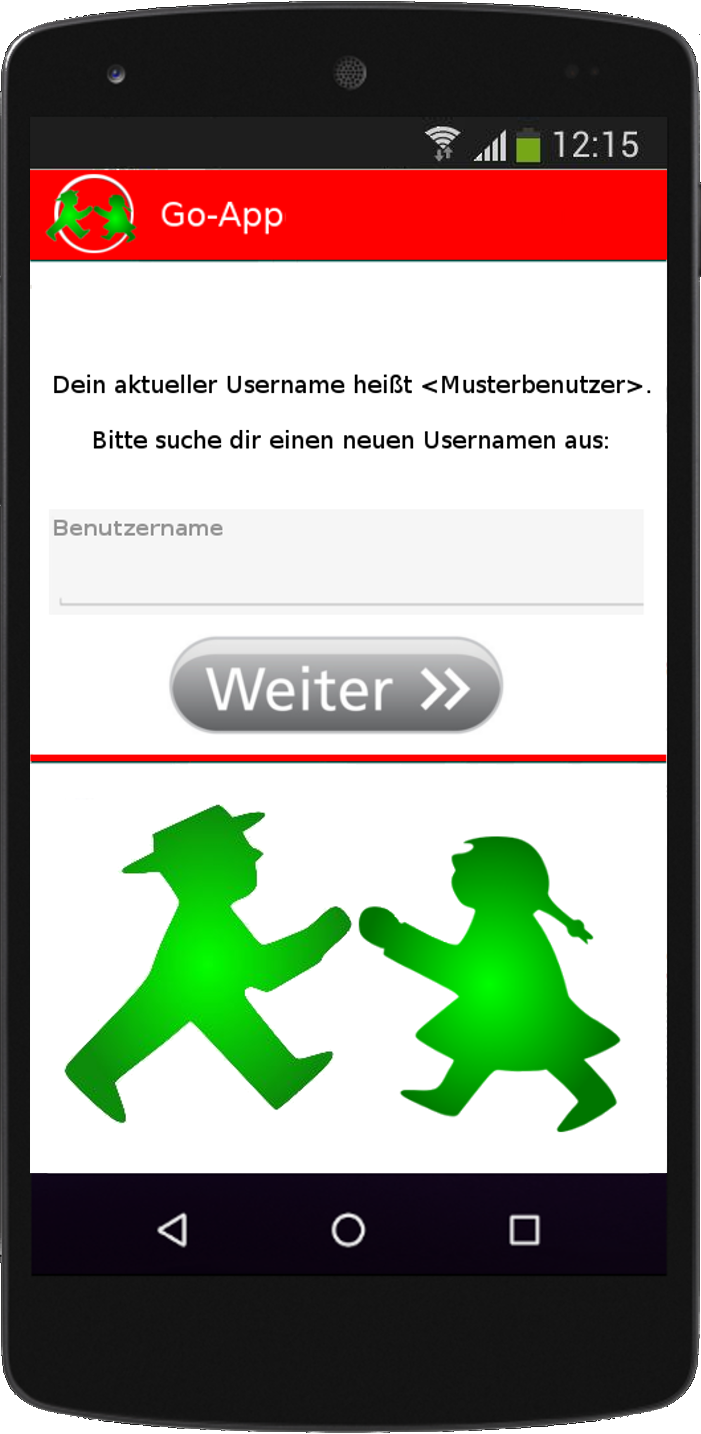
\includegraphics[scale=0.2]{resources/images/handy/username_aendern.png}
	\caption{Benutzername ändern (Wunschkriterium)}
\end{wrapfigure}

\textbf{Beschreibung:}\\
Option zum ändern des BNs(Benutzernamen), Information über den aktuellen BN und Aufforderung an den Benutzer sich einen neuen BN zu wählen.\\
\textbf{Elemente:}\\
BN zur Orientierung, mit welchem Namen der Benutzer registriert ist.\\
Textfeld "Benutzername" zum Einfügen des BNs.\\
"Weiter"-Button um diesen zu bestätigen.\\
\textbf{Verwendung:}\\
Durch einmaliges Tippen auf das Textfeld "Benutzername" wird die Bildschirmtastatur aktiviert und der Benutzer kann seinen gewählten BN eingeben.\\
Durch einmaliges Tippen auf den "Weiter"-Button wird dieser BN bestätigt und der Benutzer wird weitergeleitet zu der Gruppenübersicht.

\clearpage
 V
\section{Testfälle}
\subsection{Testfälle für Musskriterien}
%\begin{tabular}{ll}
\textbf{/T010/} Benutzer registrieren \\
\begin{itemize}
\setlength{\itemsep}{0pt}
\item Der Benutzer hat die App installiert. Dies wird über den Android Package Manager geprüft.
\item Der Benutzer registriert einen Account. Dies wird in der Datenbank des Servers geprüft.
\item Im Fehlerfall wird dem Benutzer eine Fehlermeldung angezeigt.
\end{itemize}


\textbf{/T020/} Benutzer löschen \\
\begin{itemize}
\setlength{\itemsep}{0pt}
\item Der Benutzer ist registriert. Dies wird über die auf dem Gerät
und Server gespeicherten Daten geprüft.
\item Der Benutzer löscht seinen Account. Dies wird in der Datenbank des Servers geprüft.
\item Im Fehlerfall wird dem Benutzer eine Fehlermeldung angezeigt.
\end{itemize}


\textbf{/T030/} Gruppe erstellen \\
\begin{itemize}
\setlength{\itemsep}{0pt}
\item Der Benutzer ist registriert. Dies wird über die auf dem Gerät
und Server gespeicherten Daten geprüft.
\item Der Benutzer erstellt eine Gruppe. () Dies wird in der Datenbank des Server geprüft.
\item Im Fehlerfall wird dem Benutzer eine Fehlermeldung angezeigt.
\end{itemize}

\textbf{/T040/} Gruppe löschen \\
\begin{itemize}
\setlength{\itemsep}{0pt}
\item Der Benutzer ist Administrator der Gruppe. Dies wird in der Datenbank des Servers geprüft.
\item Der Benutzer löscht die Gruppe. () Dies wird in der Datenbank des Servers geprüft.
\item Im Fehlerfall wird dem Benutzer eine Fehlermeldung angezeigt.
\end{itemize}

\textbf{/T050/} Einladung erstellen \\
\begin{itemize}
\setlength{\itemsep}{0pt}
\item Der Benutzer ist Administrator der Gruppe. Dies wird in der Datenbank des Servers geprüft.
\item Der Benutzer erstellt () und verschickt Einladungen. Dies wird in der Datenbank des Servers geprüft.
\item Im Fehlerfall wird dem Benutzer eine Fehlermeldung angezeigt.
\end{itemize}


\textbf{/T060/} Gruppe beitreten \\
\begin{itemize}
\setlength{\itemsep}{0pt}
\item Der Benutzer wurde von einem Administrator zu einer Gruppe eingeladen. ()
\item Der Benutzer tritt der Gruppe () bei. Dies wird in der Datenbank des Servers geprüft.
\item Im Fehlerfall wird dem Benutzer eine Fehlermeldung angezeigt.
\end{itemize}


\textbf{/T070/} Gruppe verlassen \\
\begin{itemize}
\setlength{\itemsep}{0pt}
\item Der Benutzer ist Mitglied der Gruppe. Dies wird in der Datenbank des Servers geprüft.
\item Der Benutzer verlässt die Gruppe. () Dies wird in der Datenbank des Servers geprüft.
\item Im Fehlerfall wird dem Benutzer eine Fehlermeldung angezeigt.
\end{itemize}


\textbf{/T080/} Aus Gruppe entfernen \\
\begin{itemize}
\setlength{\itemsep}{0pt}
\item Der Benutzer ist Administrator der Gruppe. Dies wird in der Datenbank des Servers geprüft.
\item Der Benutzer wählt ein Mitglied zum Entfernen aus. Dies wird in der Datenbank des Servers geprüft.
\item Im Fehlerfall wird dem Benutzer eine Fehlermeldung angezeigt.
\end{itemize}


\textbf{/T090/} Treffpunkt festlegen \\
\begin{itemize}
\setlength{\itemsep}{0pt}
\item Der Benutzer ist Administrator der Gruppe. Dies wird in der Datenbank des Servers geprüft.
\item Der Benutzer legt einen Treffpunkt fest. () Dies wird in der Datenbank des Servers geprüft.
\item Im Fehlerfall wird dem Benutzer eine Fehlermeldung angezeigt.
\end{itemize}


\textbf{/T100/} Go-Button drücken / Aufbrechen \\ % TODO Formulierung?
\begin{itemize}
\setlength{\itemsep}{0pt}
\item Der Benutzer ist Mitglied einer Gruppe. Dies wird in der Datenbank des Servers geprüft.
\item Ein Administrator hat einen Treffpunkt festgelegt. () Dies wird in der Datenbank des Servers geprüft.
\item Der Benutzer bricht auf / drückt den Go-Button. ()
Seine Position wird übermittelt.
Dies wird beim Server geprüft.
\item Im Fehlerfall wird dem Benutzer eine Fehlermeldung angezeigt.
\end{itemize}


\textbf{/T110/} Positionen von Gruppenmitgliedern anzeigen \\
\begin{itemize}
\setlength{\itemsep}{0pt}
\item Der Benutzer ist Mitglied einer Gruppe. Dies wird in der Datenbank des Servers geprüft.
\item Mindestens ein Mitglied ist aufgebrochen. () Dies wird in der Datenbank des Servers geprüft.
\item Der Benutzer ruft die Karte auf und sieht die Positionen der
aufgebrochenen Mitglieder. () Dies wird auf dem Gerät überprüft.
\item Im Fehlerfall wird dem Benutzer eine Fehlermeldung angezeigt.
\end{itemize}


%\end{tabular}

\subsection{Testfälle für Wunschkriterien}
\begin{tabular}{ll}
/T200/ & Aufbrechen mit aktivierten/deaktiviertem GPS-Tracking \\ % TODO Formulierung?
/T210/ & Änderung des Benutzernamens \\
/T220/ & Gruppenmitglied als zusätzlichen Administrator setzen \\
/T230/ & Änderung des Gruppennamens \\
/T240/ & Inaktive Gruppen löschen \\
/T250/ & Inaktive Benutzer löschen \\
/T260/ & Anzeigen des Aufbruchs-Status von Gruppenmitgliedern \\
/T270/ & Benachrichtigung über Aufbrechen von Gruppenmitgliedern \\
/T280/ & Benachrichtigung über Änderung des Treffpunktes \\
/T290/ & Festlegen von Treffpunkten für spezifische Zeitpunkte \\
\end{tabular}
 M
\section{Qualitätsbestimmung}
Funktionalität 
Zuverlässigkeit
Benutzbarkeit 
Effizienz 
Änderbarkeit 
Übertragbarkeit D
\section{Entwicklungsumgebung}

\subsection{Software}
Entwicklungsumgebung: 			Android Studio 2.2\\
Graphische Benutzeroberfläche: 	Android Studio 2.2\\
Versionierung: 					Git\\
Dokumentation:					LaTex\\
Betriebssystem: 				CentOS Version 6.8\\
Server:							Tomcat Version 8\\
Webserver:						Apache Version 2.2\\
Datenbankverwaltungssystem: 	MySQL Version 5.1\\
Programmiersprache:				Java 1.8\\

\subsection{Hardware} V
\section{Glossar}

Administrator/ Gruppenadministrator = Benutzer der die Gruppe erstellt hat oder von diesem zum Administrator gemacht wurde und in der Gruppe mehr Rechte besitzt als die anderen Gruppenmitglieder\\
\\
App/ Applikation/ Anwendung = Anwendungsprogramm für den Benutzer welches mindestens eine Funktion erfüllt ??? Oder was genau sollen wir da schreiben????\\
\\
Anonym = Den Standorten der Benutzers werden keine Namen zugeordnet\\
\\
Benutzer = Person welche die App geöffnet hat und gerade verwendet\\
\\
Benutzeraccount =
\\
Benutzername = Name eines Benutzers durch welchen man diesen von den anderen unterscheiden kann\\
\\
Gemittelt = Mehrere Gruppenmitglieder mit nahe beieinanderliegenden Standorten werden zu einem zusammengefasst\\
\\
Gruppe = Vereinigung mehrere Benutzer die über denselben Link beigetreten sind\\
\\
Gruppenlink = Verweis auf eine Gruppe (wird so zu einem Mitglied dieser Gruppe)\\
\\
Gruppenmitglied/ Mitglied = Alle Benutzer die derselben Gruppe angehören\\
\\
Gruppenname =
\\
Go-Button = Durch Betätigung dieses Buttons wird die Startposition des Benutzer für die anderen Gruppenmitglieder auf der Karte sichtbar\\
\\
GPS- Daten = Position eines Benutzers, wo er sich auf der Welt befindet\\
\\
Karte = Google Maps oder Open Street Map\\
\\
Produkt = Android Go-App\\
\\
Registrierung = Erstmalige Anmeldung mit festlegen eines Benutzernamens\\
\\
Standort = Die GPS Daten eines Benutzers auf der Karte\\
\\
Startposition = Der jeweilige Standort eines Benutzers in dem Moment indem er den GO-Button betätigt\\
\\
Treffpunkt = Uhrzeit und Ort eines Termins\\
\\
Zielort = Der jeweilige Standort des ausgemachten Treffpunkts\\
\\








 alle


\end{document}
